\documentclass[12pt,letterpaper]{exam}
\usepackage[lmargin=1in,rmargin=1in,tmargin=1in,bmargin=1in]{geometry}
\usepackage{../style/exams}

% -------------------
% Course & Exam Information
% -------------------
\newcommand{\course}{MATH 115: Exam 1}
\newcommand{\term}{Fall --- 2024}
\newcommand{\examdate}{09/09/2024}
\newcommand{\timelimit}{75 Minutes}

\setbool{hideans}{true} % Student: True; Instructor: False


% -------------------
% Content
% -------------------
\begin{document}

\examtitle
\instructions{Write your name on the appropriate line on the exam cover sheet. This exam contains \numpages\ pages (including this cover page) and \numquestions\ questions. Check that you have every page of the exam. Answer the questions in the spaces provided on the question sheets. Be sure to answer every part of each question and show all your work. If you run out of room for an answer, continue on the back of the page --- being sure to indicate the problem number.} 
\scores
\bottomline
\newpage


% -------------------
% Questions
% -------------------
\begin{questions}

% Question 1
\newpage
\question Let $A= [-4, 5]$, $B= (-5, 2]$, $C= [2, 6)$, and $D= (-2, 2)$. Compute the following sets: \pvspace{0.5cm}
	\begin{parts}
	\part[3] $A \cap B$ \vfill
	\part[3] $D \cup C$ \vfill
	\part[4] $(B \cup D) \cap A$ \vfill
	\end{parts}



% Question 2
\newpage
\question Consider the plot of a circle and points $A, B$ shown below. 
	\[
	\fbox{
	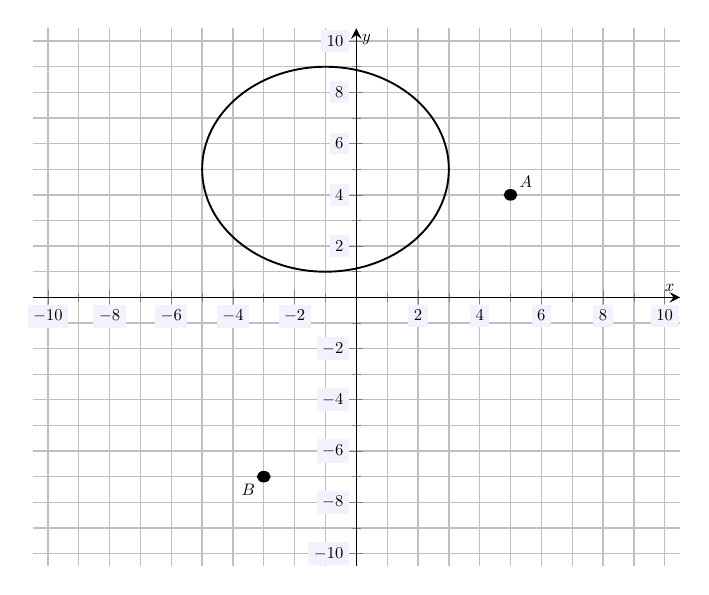
\begin{tikzpicture}[scale=1.2,every node/.style={scale=0.5}]
	\begin{axis}[
	grid=both,
	axis lines=middle,
	ticklabel style={fill=blue!5!white},
	xmin= -10.5, xmax=10.5,
	ymin= -10.5, ymax=10.5,
	xtick={-10,-8,-6,-4,-2,0,2,4,6,8,10},
	ytick={-10,-8,-6,-4,-2,0,2,4,6,8,10},
	minor tick = {-10,-9,...,10},
	xlabel=\(x\),ylabel=\(y\),
	]
	\draw[line width=0.02cm] (-1,5) circle (4);
	\draw[fill=black] (5,4) circle (0.2); \node at (5.5,4.5) {$A$};
	\draw[fill=black] (-3,-7) circle (0.2); \node at (-3.5,-7.5) {$B$};
	\end{axis}
	\end{tikzpicture}
	}
	\] 
Based on this plot, find the following: \pspace

\begin{parts}
\part[2] The distance from $A$ to the $x$-axis. \vfill
\part[2] The distance from $B$ to the $y$-axis. \vfill
\part[3] The equation of the circle. \vfill
\part[3] The distance between $A$ and $B$. \vfill
\end{parts}



% Question 3
\newpage
\question Assume that $x, y, z > 0$. Showing all your work, simplify the following as much as possible: \pvspace{0.2cm}

\begin{parts}
\part[5] $\left( \dfrac{x^{-6} y z^5}{(x^{-2} z^2)^3 y^4} \right)^{-1}$ \vfill
\part[5] $x y^5 \sqrt{\dfrac{x^7 y^{-4}}{x^3 y^8}}$ \vfill
\end{parts}



% Question 4
\newpage
\question[10] Find the linear function with $x$-intercept 8 and $y$-intercept 6. Is the point $(5, 2)$ on the graph of this function? Explain. 



% Question 5
\newpage
\question Assume that $f$ and $g$ are functions and that $f$ is one-to-one. A partial table of values for $f$ and $g$ are found below. \par
	\begin{table}[ht]
	\centering
	\begin{tabular}{|c||c|c|c|c|c|c|} \hline 
	$x$ & $-4$ & $-3$ & $\phantom{-}0$ & $1$ & $\phantom{-}2$ & $5$ \\ \hline \hline
	$f(x)$ & $\phantom{-}2$ & $\phantom{-}6$ & $-4$ & $1$ & $\phantom{-}7$ & $3$ \\ \hline
	$g(x)$ & $\phantom{-}1$ & $-5$ & $\phantom{-}2$ & $0$ & $-4$ & $6$ \\ \hline 
	\end{tabular}
	\end{table} \par
Based on the given information, compute the following: \pspace

\begin{parts}
\part[2] $(f - 2g)(2)$ \vfill
\part[2] $(fg)(-3)$ \vfill
\part[2] $(f \circ g)(0)$ \vfill
\part[2] $(g \circ f)(0)$ \vfill
\part[2] $f \left( f^{-1} \left( \sqrt{\pi} \right) \right)$ \vfill
\end{parts}



% Question 6
\newpage
\question Consider the plot of the function $f(x)= \dfrac{20 - 2x}{3}$ show below. 
	\[
	\fbox{
	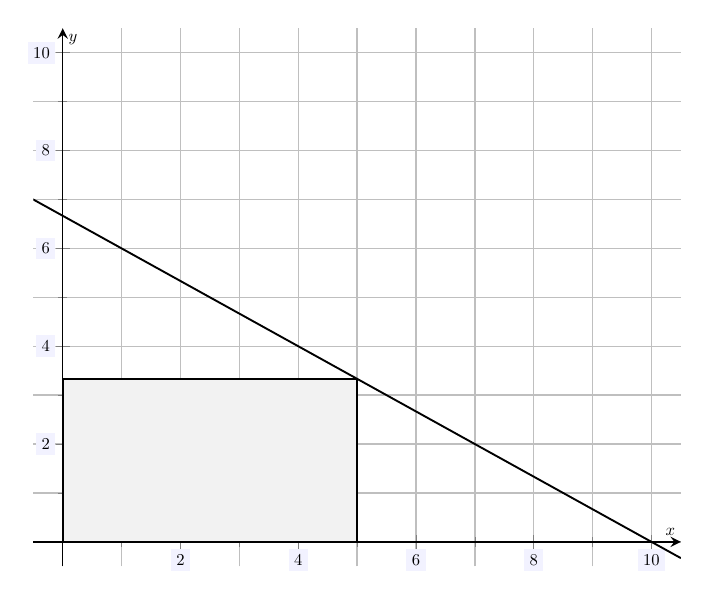
\begin{tikzpicture}[scale=1.2,every node/.style={scale=0.5}]
	\begin{axis}[
	grid=both,
	axis lines=middle,
	ticklabel style={fill=blue!5!white},
	xmin= -0.5, xmax=10.5,
	ymin= -0.5, ymax=10.5,
	xtick={-10,-8,-6,-4,-2,0,2,4,6,8,10},
	ytick={-10,-8,-6,-4,-2,0,2,4,6,8,10},
	minor tick = {-10,-9,...,10},
	xlabel=\(x\),ylabel=\(y\)
	]
	\addplot[line width= 0.02cm,samples=100,domain= -10.5:10.5] ({x},{(20 - 2*x)/3});
	\draw[line width=0.02cm,fill=gray!10] (0,0) -- (5,0) -- (5,10/3) -- (0,10/3) -- (0,0);
	\end{axis}
	\end{tikzpicture}
	}
	\] \pspace

\begin{parts}
\part[5] Find the area of the rectangle shown above. \vfill
\part[5] Find $f^{-1}(x)$. \vfill
\end{parts}



% Question 7
\newpage
\question Consider the plot of a relation $\beta$ shown below. 
	\[
	\fbox{
	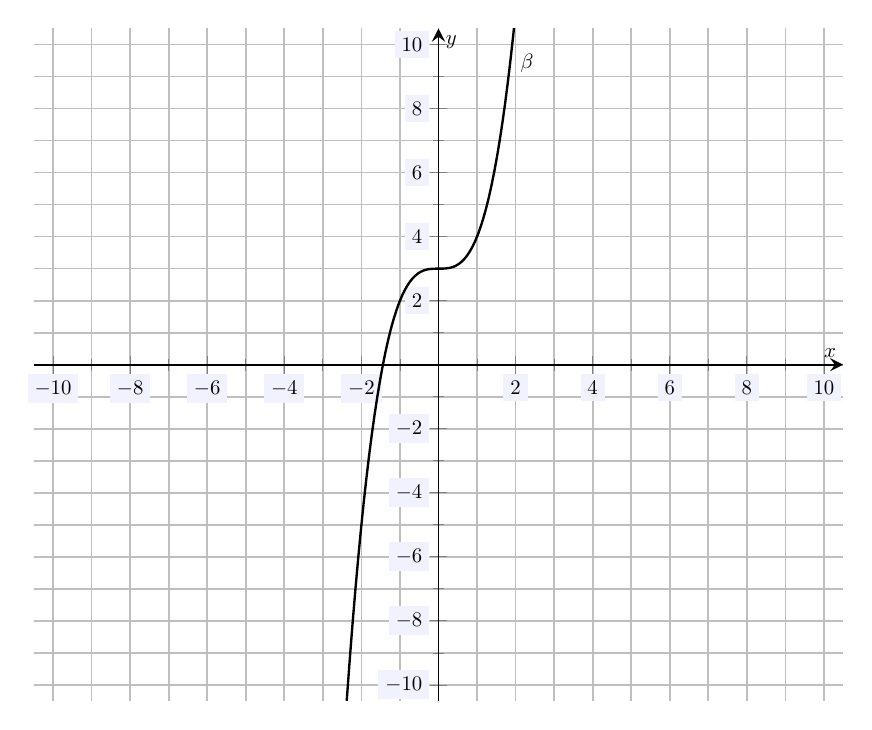
\begin{tikzpicture}[scale=1.5,every node/.style={scale=0.5}]
	\begin{axis}[
	grid=both,
	axis lines=middle,
	ticklabel style={fill=blue!5!white},
	xmin= -10.5, xmax=10.5,
	ymin= -10.5, ymax=10.5,
	xtick={-10,-8,-6,-4,-2,0,2,4,6,8,10},
	ytick={-10,-8,-6,-4,-2,0,2,4,6,8,10},
	minor tick = {-10,-9,...,10},
	xlabel=\(x\),ylabel=\(y\),
	]
	\addplot[line width= 0.02cm,samples=100,domain= -3.5:3.5] ({x},{x^3+3}); \node at (2.3,9.4) {$\beta$};
	\end{axis}
	\end{tikzpicture}
	}
	\] \pspace

\begin{parts}
\part[2] Is there an $x$ such that $\beta(x)= -5$? Explain. \vfill
\part[3] Is $\beta$ a function of $x$? Explain. \vfill
\part[5] Does $\beta^{-1}(x)$ exist? Justify your answer. If $\beta^{-1}(x)$ doe exist, sketch it on the plot above. \vfill
\end{parts}



% Question 8
\newpage
\question \textit{Butte-ane Inc.} is an oil company based out of North Dakota. An engineer at the company reports that the company is shipping the same amount of oil from their reserves each day. They also report that the amount of oil they will have in reserve tanks $d$ days from now, measured in thousands of gallons, is given by $O(d)= 168.438 - 5.3d$. 
	\begin{parts}
	\part[5] Find and interpret the slope of $O(d)$ in the context of the problem. 
	\part[5] Find and interpret the $y$-intercept of $O(d)$ in the context of the problem. 
	\end{parts}



% Question 9
\newpage
\question Sanitation workers have finished cleaning Skibidi fountain are refilling it. A hose system is feeding water into the fountain at a constant rate. After 10~minutes, the fountain will require an additional 15,400~gallons of water to fill. But after one hour, the fountain only requires 12,400~gallons. Let $W(t)$ denote the amount of water required to fill the tank after $t$ minutes. 
	\begin{parts}
	\part[5] Explain why $W(t)$ is linear.
	\part[5] Find $W(t)$. 
	\end{parts}



% Question 10
\newpage
\question[10] Determine whether the following statements are true ($T$) or false ($F$) for all real numbers $x, y, z, a, b$. Mark your answer in the space provided---no justification is necessary. \pvspace{0.5cm}
	\begin{enumerate}[(a)]
	\item \usol{0.65cm}{\itshape T}: $(x^2 + 1)^0= 1$ \vfill
	\item \usol{0.66cm}{\itshape F}: $(x + y)^2= x^2 + y^2$ \vfill
	\item \usol{0.65cm}{\itshape T}: $(x - y)^2= (y - x)^2$ \vfill
	\item \usol{0.66cm}{\itshape F}: $\dfrac{x}{y} + \dfrac{a}{b}= \dfrac{x + a}{y + b}$ \vfill
	\item \usol{0.66cm}{\itshape F}: $\dfrac{\,\,\frac{x}{y}\,\,}{z}= \dfrac{xz}{y}$ \vfill
	\item \usol{0.65cm}{\itshape T}: $\sqrt[3]{-x}= -\sqrt[3]{x}$ \vfill
	\item \usol{0.66cm}{\itshape F}: $\dfrac{x}{y} \cdot \dfrac{a}{b}= \dfrac{xb}{ya}$ \vfill
	\item \usol{0.66cm}{\itshape F}: $\sqrt{x + y}= \sqrt{x} + \sqrt{y}$ \vfill
	\item \usol{0.66cm}{\itshape F}: $\dfrac{x}{y} \cdot \dfrac{a}{b}= \dfrac{xa}{yb}$ \vfill
	\item \usol{0.65cm}{\itshape T}: $(x \cdot y)^a= x^a \cdot y^a$
	\end{enumerate}

\end{questions}
\end{document}